\documentclass{standalone}
\usepackage[dvipsnames]{xcolor}
\usepackage{tikz}
\usetikzlibrary{calc,matrix,positioning,fit,backgrounds}

\colorlet{region}{Melon}
\colorlet{complement}{SkyBlue}
\colorlet{border}{LimeGreen}

\newcommand{\pucond}{$p^{cond}_{\uparrow}$}
\newcommand{\pdcond}{$p^{cond}_{\downarrow}$}

\begin{document}
\pgfdeclarelayer{bg}
\pgfdeclarelayer{grid}
\pgfsetlayers{bg,grid,main}
\begin{tikzpicture}[
  baseline=(a),
  outline/.style={draw,ultra thick,rounded corners},
  bg/.style={rounded corners, fill},
  large/.style={inner sep=2mm},
  grid/.style={gray!50!white, thick}
]
  \matrix (lattice) [
      matrix of nodes,
      nodes={color=black,fill,minimum height=2mm,draw,circle,inner sep=0},
      column sep=9mm,
      row sep=9mm
  ]{
    ~&~&~&~\\
    ~&~&~&~\\
    ~&~&~&~\\
    ~&~&~&~\\
  };

  \begin{pgfonlayer}{grid}
    \foreach \i in {1,2,3,4} {
      \foreach \j [count=\k] in {2, 3, 4} {
        \draw[grid] ($(lattice-\i-\k)$) -- ($(lattice-\i-\j)$);
        \draw[grid] ($(lattice-\k-\i)$) -- ($(lattice-\j-\i)$);
      }
    }
  \end{pgfonlayer}

  \begin{pgfonlayer}{bg}
    %\node[outline, region, large, fit={(lattice-3-1) (lattice-1-1)}] {};
    %\node[outline, region, large, fit={(lattice-2-4) (lattice-1-1)}] {};
    \node[bg, region!30!white,large,fit={(lattice-2-4) (lattice-1-1)}] {};
    \node[bg, region!30!white,large,fit={(lattice-3-2) (lattice-1-1)}] {};

    %\node[outline, complement, large, fit={(lattice-4-1) (lattice-4-4)}] {};
    %\node[outline, complement, large, fit={(lattice-3-2) (lattice-4-4)}] {};
    \node[bg, complement!40!white, large, fit={(lattice-4-1) (lattice-4-4)}] {};
    \node[bg, complement!40!white, large, fit={(lattice-3-3) (lattice-4-4)}] {};

    \node[outline, ultra thick, border, dashed, large, fit={(lattice-3-1) (lattice-3-2)}] {};
    \node[outline, ultra thick, dashed, border, large, fit={(lattice-2-3) (lattice-2-4)}] {};
  \end{pgfonlayer}

  \node [above right=2mm and 2mm of lattice-2-1] {$X$};
  \node [below=1mm of lattice-2-3] {$\partial X$};
  \node [above right=2mm and 2mm of lattice-4-3] {$\overline{X}$};
  \node at (current bounding box.north west) [anchor=south east] (a) {\textbf{a.}};
\end{tikzpicture}
\hspace{1cm}
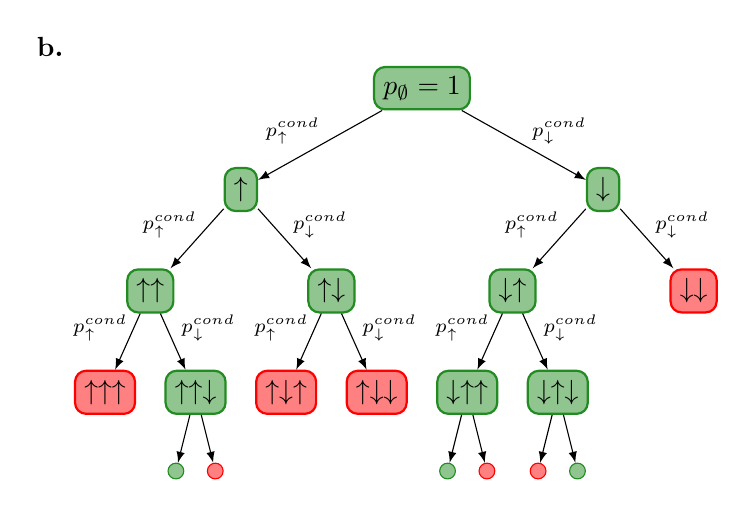
\begin{tikzpicture}[
      baseline=(b),
      level 1/.style={sibling distance=4.6cm},
      level 2/.style={sibling distance=2.3cm},
      level 3/.style={sibling distance=1.15cm},
      level 4/.style={sibling distance=5mm},
      nonleaf/.style={draw,thick,rounded corners,anchor=north},
      leaf/.style={circle, minimum width=2mm,inner sep=0, fill},
      accept/.style={draw=ForestGreen, fill=ForestGreen!50!white},
      drop/.style={draw=red, fill=red!50!white},
      edge from parent/.style={draw,-latex},
      label/.style={inner sep=0,font={\scriptsize}},
      rlab/.style={label,right=1mm,anchor=south west},
      llab/.style={label,left=0,anchor=south east},
      level distance=1cm
  ]
  \node[nonleaf, accept] {$p_{\emptyset}=1$}
  child {
    node[nonleaf, accept] {$\uparrow$}
    child {
      node[nonleaf, accept] {$\uparrow\uparrow$}
      child {
        node[nonleaf, drop] {$\uparrow\uparrow\uparrow$}
        edge from parent node[llab] {\pucond}
      }
      child {
        node[nonleaf, accept] {$\uparrow\uparrow\downarrow$}
        child {
          node[leaf, accept] {}
        }
        child {
          node[leaf, drop] {}
        }
        edge from parent node[rlab] {\pdcond}
      }
      edge from parent node[llab] {\pucond}
    }
    child {
      node[nonleaf, accept] {$\uparrow\downarrow$}
      child {
        node[nonleaf, drop] {$\uparrow\downarrow\uparrow$}
        edge from parent node[llab] {\pucond}
      }
      child {
        node[nonleaf, drop] {$\uparrow\downarrow\downarrow$}
        edge from parent node[rlab] {\pdcond}
      }
      edge from parent node[rlab] {\pdcond}
    }
    edge from parent node[llab] {\pucond}
  }
  child {
    node[nonleaf, accept] {$\downarrow$}
    child {
      node[nonleaf, accept] {$\downarrow\uparrow$}
      child {
        node[nonleaf, accept] {$\downarrow\uparrow\uparrow$}
        child {
          node[leaf, accept] {}
        }
        child {
          node[leaf, drop] {}
        }
        edge from parent node[llab] {\pucond}
      }
      child {
        node[nonleaf, accept] {$\downarrow\uparrow\downarrow$}
        child {
          node[leaf, drop] {}
        }
        child {
          node[leaf, accept] {}
        }
        edge from parent node[rlab] {\pdcond}
      }
      edge from parent node[llab] {\pucond}
    }
    child {
      node[nonleaf, drop] {$\downarrow\downarrow$}
      edge from parent node[rlab] {\pdcond}
    }
    edge from parent node[rlab] {\pdcond}
  };
  \node at (current bounding box.north west) [anchor=south east] (b) {\textbf{b.}};
\end{tikzpicture}
\end{document}
